\documentclass[tikz,border=8pt]{standalone}
\usetikzlibrary{arrows.meta,angles,quotes}
\begin{document}
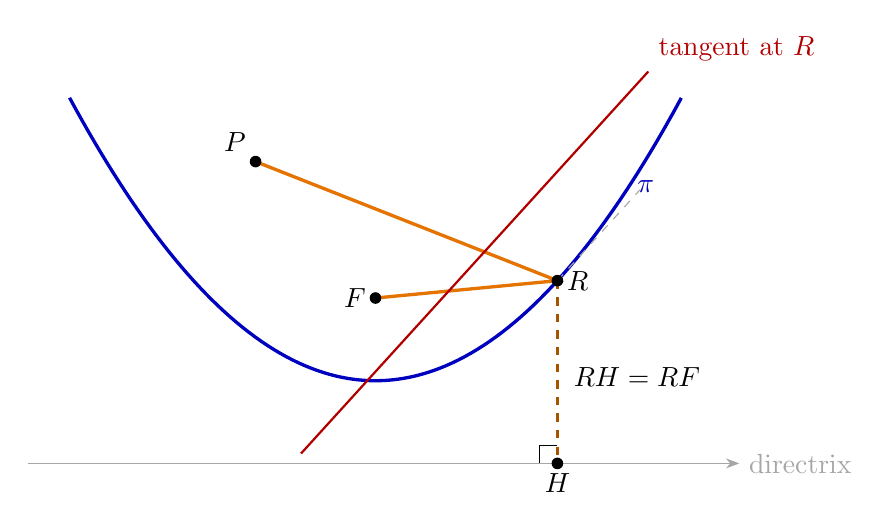
\begin{tikzpicture}[>=Stealth,scale=1.05]
  \draw[->,gray!70] (-4.2,0) -- (4.4,0) node[right] {directrix};
  \draw[blue!75!black,very thick,domain=-3.7:3.7,samples=100]
    plot (\x,{1 + (\x*\x)/4});
  \node[blue!75!black,right] at (3.05,3.35) {$\pi$};

  \coordinate (F) at (0,2);
  \coordinate (P) at (-1.45,3.65);
  \coordinate (R) at (2.2,2.21);
  \coordinate (H) at (2.2,0);
  \coordinate (T) at (3.2,3.31);

  \draw[orange!90!black,very thick] (P) -- (R) -- (F);
  \draw[orange!65!black,dashed,thick] (R) -- (H);
  \draw[gray!70,dashed] (R) -- (T);
  \draw[red!70!black,thick] (-0.9,0.12) -- (3.3,4.74) node[above right] {tangent at $R$};

  \fill (F) circle (2pt) node[left] {$F$};
  \fill (P) circle (2pt) node[above left] {$P$};
  \fill (R) circle (2pt) node[right] {$R$};
  \fill (H) circle (2pt) node[below] {$H$};
  \node[right] at (2.28,1.05) {$RH=RF$};
  \draw (2.2,0.22) -- (1.98,0.22) -- (1.98,0);
\end{tikzpicture}
\end{document}
